% arara: pdflatex
% !arara: biber
% !arara: pdflatex
% How to run: 
% 1) pdflatex "filename".tex
% 2) biber "filename"
% 3) pdflatex "filename".tex
% 4) pdflatex "filename".tex


\documentclass[x11names]{article}
\usepackage{verbatim}
\usepackage{listings}
\usepackage{graphicx}
\usepackage{a4wide}
\usepackage{color}
\usepackage{amsmath}
\usepackage{amssymb}
\usepackage[dvips]{epsfig}
\usepackage[T1]{fontenc}
% \usepackage{cite} % [2,3,4] --> [2--4]
\usepackage{shadow}
\usepackage{hyperref}
\usepackage{physics}
\usepackage{url}
%For use in pictures
\usepackage{tikz}
\usepackage{tikz-3dplot}
\usepackage{wrapfig}


\usepackage{subcaption}
\usepackage[utf8]{inputenc}
\usepackage{booktabs} % Allows the use of \toprule, \midrule and \bottomrule in tables
\usepackage[font={small,it}]{caption}
\usepackage[margin=0.7in]{geometry} %Sets the margins in the document
\usepackage{siunitx}    %Allows use of SI units macros

%Defines calculator way to write powers of ten
\sisetup{output-exponent-marker=\textsc{e}}
\renewcommand{\va}{\vec}


% Change numbering and some commands
\renewcommand\thesection{Exercise \Roman{section}}
\renewcommand\thesubsection{\Roman{section}.\alph{subsection}}

%% references
\usepackage[style=authoryear,
            bibstyle=authoryear,
            backend=biber,
            % refsection=chapter,
            maxbibnames=99,
            maxnames=2,
            firstinits=true,
            uniquename=init,
            natbib=true,
            dashed=false]{biblatex}

\addbibresource{bibliography.bib}
% \addbibresource{top.bib}

% \bibliography{bibliography}
% \bibliography{top}


\usepackage[capitalize]{cleveref}

\setcounter{tocdepth}{2}

\lstset{language=c++}
\lstset{alsolanguage=[90]Fortran}
\lstset{basicstyle=\small}
\lstset{backgroundcolor=\color{white}}
\lstset{frame=single}
\lstset{stringstyle=\ttfamily}
\lstset{keywordstyle=\color{red}\bfseries}
\lstset{commentstyle=\itshape\color{blue}}
\lstset{showspaces=false}
\lstset{showstringspaces=false}
\lstset{showtabs=false}
\lstset{breaklines}


\definecolor{keywords}{RGB}{255,0,90}
      \definecolor{comments}{RGB}{0,0,113}
      \definecolor{red}{RGB}{160,0,0}
      \definecolor{green}{RGB}{0,150,0}
       
      \lstset{language=Python, 
              basicstyle=\ttfamily\small, 
              keywordstyle=\color{keywords},
              commentstyle=\color{comments},
              stringstyle=\color{red},
              showstringspaces=false,
              identifierstyle=\color{green}
              }



\title{ Exercise 6 \\ Sommerjobb Numeriske Plasmaoppgaver }
\author{Gullik Vetvik Killie
		}


%%%%%%%%%%%%%%%%%%%%%%%%%%%%%%%%%%%%%%%%%%%%%%%%%%%%%%%%%%%%%%%%%%%%%%%%%%%%%%%%%%%%
% Actual text starts here
%%%%%%%%%%%%%%%%%%%%%%%%%%%%%%%%%%%%%%%%%%%%%%%%%%%%%%%%%%%%%%%%%%%%%%%%%%%%%%%%%%%%
\begin{document}


\maketitle

\section{}

\subsection{Theory}
  Now we want to look at the currents aligned with the background magnetic field \( \va{B}_0 \), FACs. These currents appear as a consequence of the E-cross-B driven currents, since the E-cross-B currents will feel a Lorentz force perpendicular to the currents and the magnetic field.


  The height integrated currents perpendicular to the magnetic field is given by 

  \begin{align}
    \va{I}_\perp &= \Sigma_P \va{E} + \Sigma_H \frac{\va{E}\cross \va{B}_0}{B_0}
  \end{align}

  where \(\Sigma_P\) and \(\Sigma_H\) is the height integrated Pedersen and Hall conductances, while \(\va{E}\) is the electric field. If we take the divergence of the total perpendicular current we obtain the parallel current, due to continuity.

  \begin{align}
    \va{j}_\parallel &= \nabla \cdot \va{I}_\perp = \nabla \cdot (\Sigma_P \va{E}) + \nabla \cdot \left(\Sigma_H \frac{\va{E}\cross \va{B}_0}{B_0}\right)
    \intertext{Assuming homogeneous conductances, \(\nabla\Sigma_P = \nabla\Sigma_H = 0\)}
    \va{j}_\parallel &= \Sigma_P\nabla \cdot \va{E} + \Sigma_H \nabla \cdot \left(\frac{\va{E}\cross \va{B}_0}{B_0}\right)
    \intertext{Given \( \nabla \cdot \left(\va{E}\cross \va{B}_0 \right) = 0\) the parallel current is given by}
    \va{j}_\parallel &= \Sigma_P\nabla \cdot \va{E}
    \intertext{Then we use the relation between the E-cross-B drift and the electric field, \( \va{v} = \frac{\va{E}\cross \va{B}_0}{B_0 ^2}\), cross both sides with \(\va{B}_0\) and we arrive at  \( \va{E} = -\va{v}\cross \va{B}_0\) which we insert into expression for the parallel current.}
    \va{j}_\parallel &= \Sigma_P \nabla \cdot \left( -\va{v} \cross \va{B}_0 \right)
    \\
    &= -\Sigma_P \nabla \va{B}_0 \cdot \left( \nabla \cross \va{v} \right) + \Sigma_P \nabla \va{v} \cdot \left( \nabla \cross \va{B}_0 \right)
    \intertext{Neglecting the term containing the curl of the magnetic field we get a term for field aligned current}
    \va{j}_\parallel &= \Sigma_P \va{B}_0 \cdot \left( \nabla \cross \va{v}  \right) \label{eq:FACs}
  \end{align}

  In the last exercise calculated the plasma drift in the upper latitudes, from the electrostatic potential, we will now use this to compute the FACs according to \cref{eq:FACs}, letting \( \Sigma_P = 1\).

  Since the magnetic field is radially directed we only need the radial part of the curl of the velocity which is

  \begin{align}
    ( \nabla \cross \va{v} )_r &= \frac{1}{r\sin( \theta )} \left(  \pdv{}{\theta} (v_\phi \sin\theta) - \pdv{v_\theta}{\phi} \right)
    \intertext{Let us use the same discretization scheme as earlier and introduce the notation \(\va{v}( \theta + \differential \theta , \phi) = \va{v}_{i + 1, j}\)}
    ( \nabla \cross \va{v} )_r &\approx \frac{1}{r\sin( \theta_{i,j} )} \left(  \frac{v_{\phi, i + 1, j} \sin(\theta_{i + 1, j})   -  v_{\phi, i - 1, j} \sin(\theta_{i - 1, j}) }{2\Delta \theta  } - \frac{v_{\theta,i,j + 1} - v_{\theta,i,j-1}}{2\Delta \phi} \right)
  \end{align}

  \subsection{Results}

  Should this make any sense?

  \begin{figure}
    \centering
    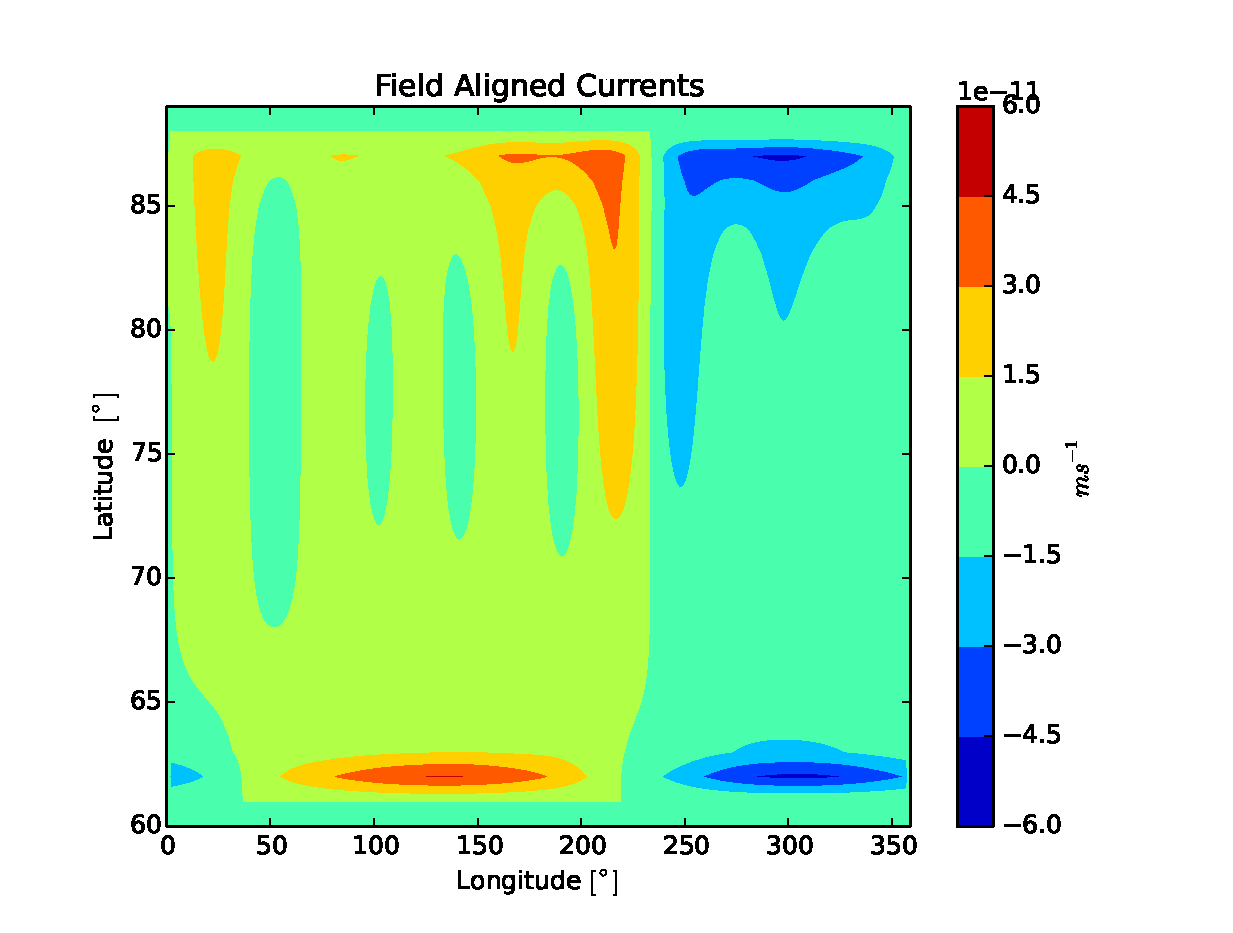
\includegraphics[width = \textwidth]{../source/facs}
    \caption{The field aligned currents as produced by the curl of the perpendicular velocities}
    \label{fig:FACs}
  \end{figure}


\appendix
\section{Comments to Exercise}
  
  \begin{itemize}
    \item Noone yet
  \end{itemize}



\section{Code}
  \label{sec:code}
  \lstinputlisting{../source/facs.py}


\end{document}